\section{Environment Models}
\label{sec:environment}

The environment module (\texttt{Environement.py}) is a pure service layer:
it supplies the world the vehicle flies through and never calls back into
vehicle, dynamics or control code. Its services are the standard atmosphere,
point-mass gravity with its gradient, the acceleration of the rotating
Earth-fixed frame, the wind, and the ground reference; all evaluations are
stateless functions of the current state. Following the project convention,
any state outside a modeled domain is rejected with an error, never
extrapolated.

\subsection{Atmosphere}

The atmosphere follows the US Standard Atmosphere 1976 \cite{ussa1976}:
seven gradient layers between sea level and the mesopause at
$84.852\,\mathrm{km}$, reproduced layer by layer. Within a layer with base
temperature $T_b$, base pressure $p_b$ and lapse rate $L$, and in the
isothermal case, the pressure is
%
\begin{equation}
\label{eq:atmosphere-pressure}
p(h) = p_b \left( \frac{T_b + L\,(h - h_b)}{T_b} \right)^{-\frac{g_0}{R\,L}}
\quad (L \neq 0),
\qquad
p(h) = p_b \, \exp \left( -\frac{g_0\,(h - h_b)}{R\,T_b} \right)
\quad (L = 0),
\end{equation}
%
with $g_0 = 9.80665\,\mathrm{m/s^2}$ and the gas constant of dry air
$R = 287.05287\,\mathrm{J/(kg\,K)}$. Density and speed of sound follow the
ideal-gas and isentropic relations,
$\rho = p/(R\,T)$ and $a = \sqrt{\gamma R T}$ with $\gamma = 1.4$.
Sea-level values are $T = 288.15\,\mathrm{K}$,
$p = 101\,325\,\mathrm{Pa}$, $\rho = 1.225\,\mathrm{kg/m^3}$.

Above the mesopause the model deliberately stops claiming physics: an
isothermal tail at $T_m = 186.946\,\mathrm{K}$ decays exponentially with a
scale height of $R\,T_m/g_0 \approx 5.47\,\mathrm{km}$ toward numerical
vacuum (density below $10^{-150}\,\mathrm{kg/m^3}$ at the
$2\,000\,\mathrm{km}$ envelope ceiling; $p(200\,\mathrm{km}) \approx
2.7\times10^{-10}\,\mathrm{Pa}$). The envelope
$0$--$2\,000\,\mathrm{km}$ is the mission scope; altitudes outside raise a
domain error instead of a number. Figure~\ref{fig:environment-models}
shows the model against the published USSA 1976 checkpoint values that the
test suite pins ($5$--$80\,\mathrm{km}$, altitudes, temperatures,
pressures and densities compared at $5\times10^{-5}$ relative tolerance).
The environment suite of $41$ tests additionally checks layer-boundary
continuity, monotone pressure and density decay, exact tail scale height,
and hydrostatic balance $\partial p/\partial h = -g_0\,\rho$ inside every
layer.

\begin{figure}[htbp]
\centering
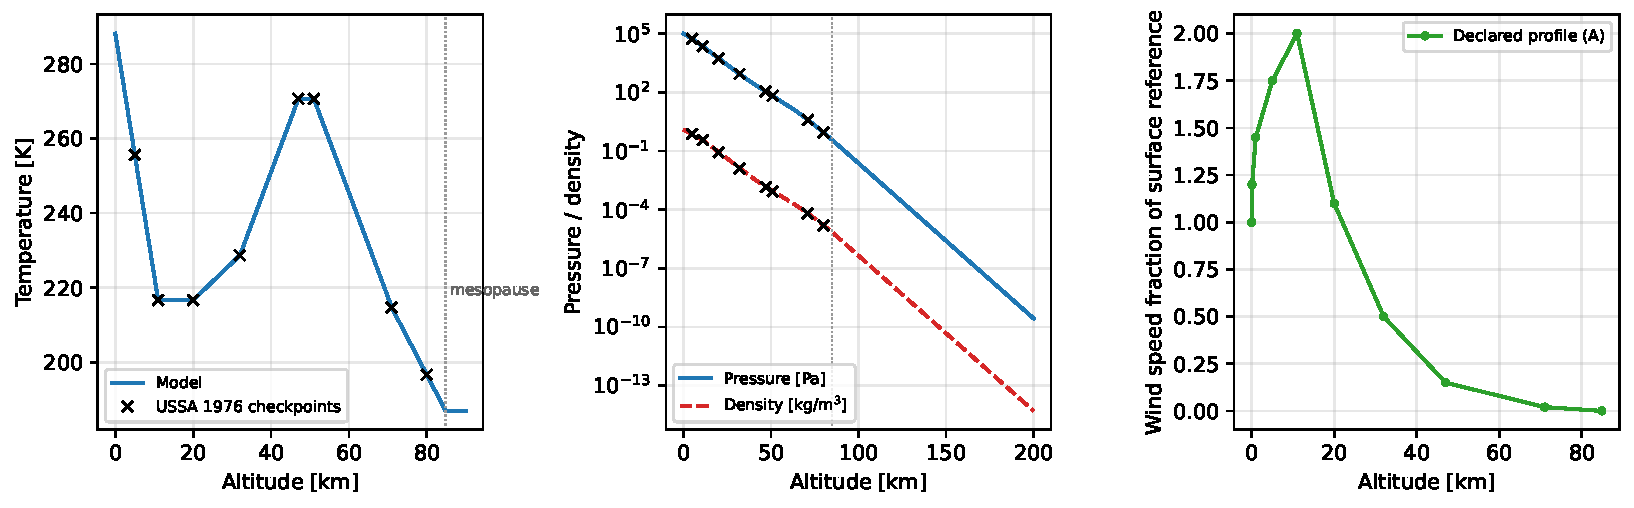
\includegraphics[width=\linewidth]{images/environment_models.pdf}
\caption{Environment model. Left: layer temperatures to the mesopause
with published USSA 1976 checkpoint values. Center: pressure and density
(logarithmic) to $200\,\mathrm{km}$, showing the isothermal tail above
the mesopause; black markers are the published checkpoints. Right: the
declared wind-profile scale factor of the surface reference wind (class
A), which is zero above the modeled atmosphere; the nominal mission runs
in calm air.}
\label{fig:environment-models}
\end{figure}

\subsection{Gravity and rotating-frame accelerations}

Gravity is the reduced Newtonian point-mass model. With the Earth radius
$R_E = 6\,371\,\mathrm{km}$ and the configured surface gravity $g_0$, the
gravitational parameter is $\mu = g_0 R_E^2$, so the gravitational
acceleration at the launch site is the configured value by construction:
%
\begin{equation}
\label{eq:gravity}
\mathbf{a}_g = -\,\frac{\mu}{\|\mathbf{r}\|^3}\,\mathbf{r}.
\end{equation}
%
Gravity never appears as a force; Equation~\eqref{eq:gravity} is added
once as an acceleration next to thrust over mass. The module also provides
the $3\times3$ gravity-gradient map
$\nabla_{\mathbf{r}}\mathbf{a}_g = (\mu/\|\mathbf{r}\|^3)\,
(3\,\hat{\mathbf{r}}\hat{\mathbf{r}}^{\mathsf{T}} - \mathbf{I})$, used only
in the navigation filter's prediction Jacobian (the navigation chapter),
not for torques. Oblateness ($J_2$) is out of scope.

The external frame is Earth-centred and launch-aligned (detailed in the
reference-frames chapter of this report); it does not rotate for the
flight mechanics themselves. Earth rotation enters translation only,
through the separate frame acceleration
%
\begin{equation}
\label{eq:frame-acceleration}
\mathbf{a}_{\mathrm{fr}} = -2\,\boldsymbol{\omega}_E \times \mathbf{v}
\;-\; \boldsymbol{\omega}_E \times
(\boldsymbol{\omega}_E \times \mathbf{r}),
\end{equation}
%
the Coriolis and centrifugal terms for velocity relative to the rotating
Earth, with the rotation vector
$\boldsymbol{\omega}_E = \Omega\,(\cos\varphi,\, 0,\, \sin\varphi)$ at
launch latitude $\varphi$. The nominal mission uses the sidereal rate
$\Omega = 7.2921150\times10^{-5}\,\mathrm{rad/s}$ at
$\varphi = 28.6^{\circ}$; setting $\Omega = 0$ disables the terms. The
frame accelerations, and their analytical gradients, are supplied once
per integration step next to gravity. The angular equations and the gyro
model retain the project's approximate Earth-rate treatment: no complete
inertial-rate coupling is claimed.

\subsection{Wind and ground reference}

The wind model is a surface reference vector (ECEF components in the
mission configuration) that can be rotated about the launch-site vertical,
scaled by a declared altitude profile: the scale factor of the surface
reference grows through the boundary layer, peaks at $2.0$ around the
$11\,\mathrm{km}$ jet-stream core, decays through the stratosphere and
reaches exactly zero at the mesopause --- there is no wind above the
modeled atmosphere (Figure~\ref{fig:environment-models}, right). The
profile is a declared stylization (class A). There are no gusts, no time
dependence and no direction shear, and the wind enters the physics only
through the relative-velocity term of the aerodynamics model. The nominal
full-mission run uses calm air: the mission configuration sets no surface
reference wind, so the default zero vector applies throughout.

The ground is a bare sphere of radius $R_E$; altitude is measured radially
above it, with an optional reference-level shift, and supports a station
offset from the center of gravity (used, for example, for engine-exit
altitude). Terrain and contact forces are out of scope; contact is
evaluated at the mission level through the leg-tip geometry discussed with
the landing criteria in the return-control chapter of this report.

The module validates its configuration at construction: non-finite
gravity, radius, ground offset or wind, non-positive radius, a negative
rotation rate or a latitude beyond $\pm 90^{\circ}$ all raise an error
before flight, not mid-integration.
